\chapter{Классификация эмоций}
Одной из главных проблем в исследованиях, связанных с определением эмоционального состояния диктора по голосу, является отсутствие четкого определения эмоции. При формализации этого понятия возникают сложности в силу многообразия психологических моделей эмоциональных процессов. Подход к классификации эмоций влияет на процесс аннотирования -- разметки аудиовизуального эмоционально окрашенного контента. 

Для формализации эмоциональных данных необходимо сформировать полноценную классификацию эмоциональных состояний, от которой в том числе напрямую зависит процесс аннотирования -- сопоставления инофрмативных признаков, полученных из речи диктора с определенными эмоциями и аффективными состояниями.

Сегодня широко используются три подхода : дискретная, многомерная и гибридная модель.

\section{Дискретная модель эмоциональной сферы}
Дискретный подход основан на выделении фундаментальных (базовых) эмоций, сочетания которых порождают разнообразие эмоциональных явлений. Разные авторы называют разное число таких эмоций -- от двух до десяти. П.~Экман на основе изучения лицевой экспрессии выделяет пять базовых эмоций: гнев, страх, отвращение, печаль и радость. Первоначальная версия 1999 года также включала <<удивление>> \cite{Ekman1972, Ekman1992}. Р.~Плутчик \cite{Plutchik1980} выделяет восемь базисных эмоций, деля их на четыре пары, каждая из которых связана с определенным действием: страх, уныние, удивление и т.~д. На рисунке \ref{fig:emo-atlas} представлена схема классификации эмоций, предложенная П.~Экманом. 

На сегодняшний день концепция существования базовых эмоций ставится под сомнение. Теория встречает ряд концептуальных проблем, таких как, например, эмпирическое определение набора базовых эмоций или критерии синхронизации эмоциональных реакций. Однако, многие решения в области автоматического детектирования эмоций основаны на дискретной модели эмоциональной сферы. Например, решение компании Affectiva \cite{Affectica}.

\begin{figure}[H]
	\centering
	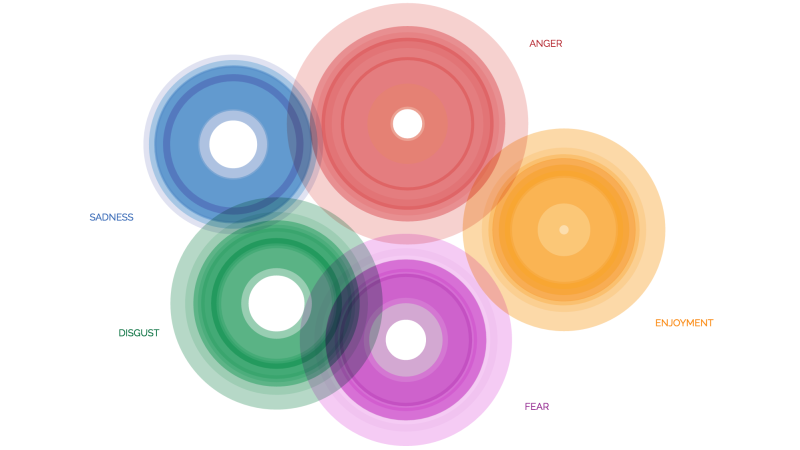
\includegraphics[width=\linewidth]{assets/emo-atlas}
	\caption{Атлас эмоций, предложенный П.~Экманом}
	\label{fig:emo-atlas}
\end{figure}

\section{Многомерная модель эмоциональной сферы}
Многомерная модель представляет собой эмоции в координатном многомерном пространстве. В качестве ее источника рассматривают идею В. Вундта о том, что многогранность чувств
человека можно описать с помощью трех измерений: удовольствие~-~неудовольствие, расслабление~-~напряжение, возбуждение~-~успокоение. Вундт заключил, что эти измерения охватывают все разнообразие эмоциональных состояний \cite{Вундт1984}. Данные для этой теории были получены с помощью метода интроспекции.

Эмоциональная сфера представляется как многомерное пространство, образованное некоторым
количеством осей координат. Оси задаются полюсами первичных характеристик эмоций. Отдельные эмоции -- это точки, местоположение которых в <<эмоциональном>> пространстве определяется степенью выраженности этих параметров.

Один из примеров описываемого подхода -- модель Дж. Рассела. В ней водится двумерный базис, в котором каждая эмоция характеризуется знаком (\textit{valence}, валентность) и интенсивностью (\textit{arousal}, активацией). Измерение валентности отражает то,
насколько хорошо человек ощущает себя на уровне субъективного переживания от максимального неудовольствия до максимального удовольствия. Измерение активации связано с
субъективным чувством энергии и ранжируется в диапазоне от дремоты до бурного возбуждения. Такой подход используется, например, в датасете RECOLA \cite{RECOLA}.

Аналогично вопросу о количестве эмоций в дискретной модели, вопрос о количестве измерений остается открытым. Использование только двух критикуется на том основании, что они не позволяют устанавливать различия между отдельными эмоциональными состояниями (например, страх, гнев, ревность, презрение и др. имеют отрицательную валентность и высокую активацию).

\section{Гибридная модель эмоциональной сферы}
Гибридная модель представляет собой комбинацию дискретной и многомерной модели. Примером такой модели являются <<Песочные часы эмоций>>, предложенные Камбрией, Ливингстоном, Хуссейном \cite{hourglass}. 
\begin{figure}[H]
	\centering
	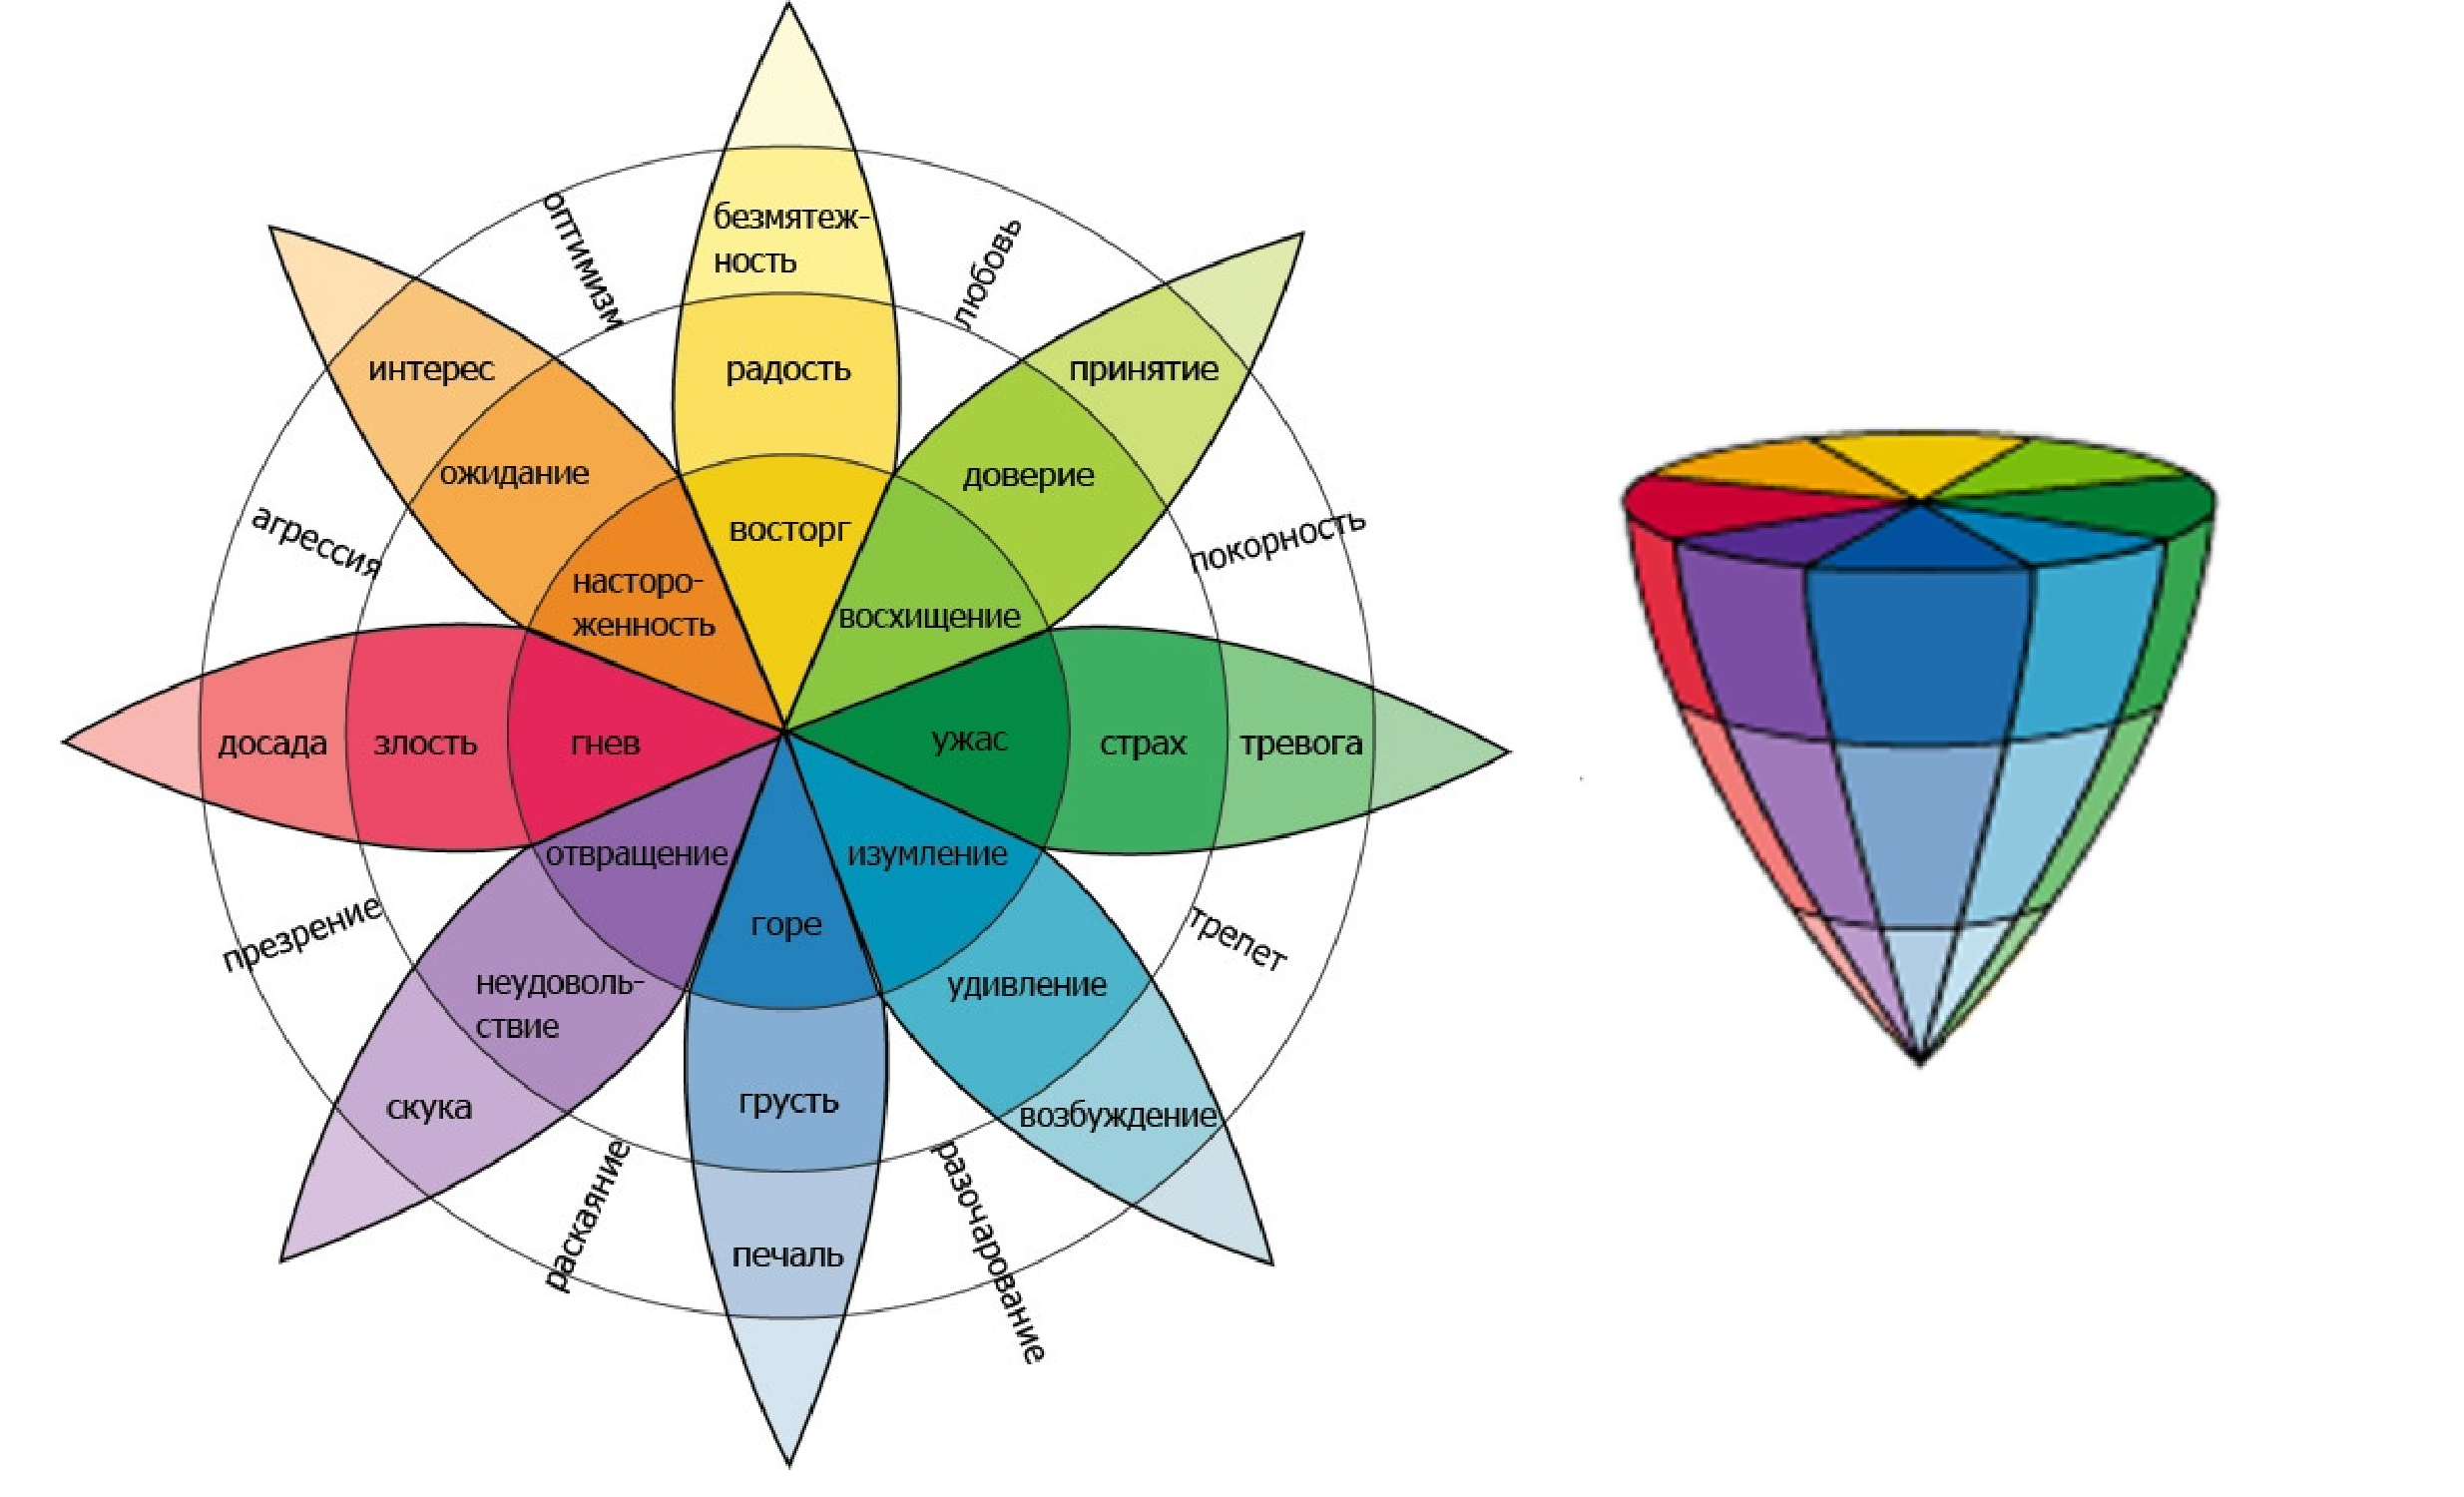
\includegraphics[width=0.8\linewidth]{assets/hourglass.pdf}
	\caption{Трехмерная модель Роберта Плутчика, в основании которой лежим круговая траектория фундаментальных эмоций (слева)}
	\label{fig:hourglass}
\end{figure}

Согласно этой классификации, в отдельной области $n$~-мерного эмоционального пространства различия между эмоциями могут определяться в терминах измерений, имеющих отношение к этой области. Эмоции могут быть сопоставимы по измерениям внутри и вне категорий, и каждая категория может иметь свои отличительные признаки \cite{Russell2003}. Каждое измерение характеризуется шестью уровнями силы, с которой выражены эмоции. Данные уровни обозначаются набором из двадцати четырех эмоций. Поэтому совершенно любая эмоция может рассматриваться как и фиксированное состояние, так и часть пространства, связанная с другими эмоциями нелинейными отношениями. 

Выбор подхода от цели. Многомерные модели позволяют избежать проблемы существования  некоторых слов в каких-то языках, в то время как в других может не быть слов для описания этих эмоций. Это делает процесс аннотирования культурно-зависимым. Тем не менее разные аннотаторы дают разные оценки выраженности валентности или активации, поэтому в целях упрощения модели для некоторых задач больше подходит дискретная модель.

\chapter[Информативные признаки, характеризующие речь]{Информативные признаки, характеризующие речь}
Условно характеристики речи диктора можно разбить на два основных
класса -- \textit{акустические} и \textit{лингвистические}. В зависимости от решаемой задачи
их относительная эффективность может быть различной. \cite{speech-patterns}

 Акустические характеристики голоса могут быть условно разделены на пять категорий \cite{categories}:
\begin{itemize}
	\item просодические;
	\item фонационные (отношение гармоник основного тона к шуму, джиттер, шиммер);
	\item динамические;
% 	\item динамические (фонетическая функция \cite{phonetic-func}, отношение гармоник основного тона к шуму \cite{phonetic-func-1}, $\cdots$);
	\item спектральные;
	\item энергетические (отношение мощностей в спектральных полосах, оценка мощности сигнала).
\end{itemize}

\noindentКаждая группа показателей находит свое применение в описании отдельных аспектах голоса, являющихся показателями различных эмоциональных состояний. На ранних этапах развития систем детектирования эмоций информативность параметров определялась эвристически. В настоящем используются алгоритмы отбора информативных признаков. Существует два класса алгоритмов: <<обертки>> и  <<фильтры>>.

Обертка, или \textit{wrapper based selection} использует оценку работы классификатора в качестве критерия оптимизации внутри замкнутого цикла. Примером является стратегия линейного последовательного поиска -- алгоритм начинает с пустого множества и последовательно
добавляет к нему наилучшие информативные признаки. \cite{wrapper}

<<Фильтры>> основаны на методах теории информации либо корреляционном анализе. Критерием оптимизации является некоторая функция, соотносящаяся с корреляциями между информативными признаками, приростом информации при их  добавлении к набору, определенными метриками в пространстве признаков и статистиками. \cite{filter}

\section{Просодические характеристики}

Просодические характеристики -- это совокупность темпорального, артикуляционного и интонационного ее компонентов. В таблице \ref{tab:pro} представлены основные просодические параметры речевого сигнала, связанные с эмоциональным состоянем человека. \cite{params}

\newcolumntype{G}{>{\centering}p{0.3\textwidth}}
\newcolumntype{C}{>{\centering\arraybackslash}p{0.3\textwidth}}

\begin{table}[H]
    \centering
        \caption{Соответствие между просодическими особенностями речи и эмоциональным состоянием}
        \label{tab:pro}
        \begin{tabular}{GCC}
            \hline
            \textit{параметры} & \textit{высокое значение} & \textit{низкое значение} \\ \hline
            изменчивость частоты основного тона & радость, гнев, страх & печаль, безразличие \\ \hline
            уровень частоты основного тона & радость, гнев, страх, чувство приподнятости и уверенности в себе & печаль, презрение, скука, безразличие \\ \hline
            интенсивность & радость, гнев, презрение, чувство приподнятости, уверенности в себе, силы, эмоциональное оценивание & печаль, презрение, скука, безразличие \\ \hline
            темп & радость, гнев, страх, чувство приподнятости, уверенности в себе, безразличия & печаль, презрение, скука \\ \hline
    \end{tabular}
\end{table}

Наиболее устойчивыми при создании системы распознавания эмоций являются изменчивость частоты основного тона и темп, использование параметра интенсивности связано с аппаратурными параметрами ввода сигнала в систему обработки, поэтому необходимо использовать некоторую относительную величину, например, отношение интенсивности гласных и согласных звуков. \cite{params-eff}

\section{Спектральные характеристики}
Спектральная группа характеристик основана на преобразовании Фурье. В частности, мел-частотный анализ.

Мел-частотный анализ представляет частоты речи с позиции психоакустического параметра слуха -- высоты тона. \cite{mel} Высота тона определяет, насколько высоким или низким кажется тон слушателю. Нелинейную связь между частотой звука и его высотой отображает мел-частотная шкала (рисунок \ref{fig:mel-hz}).

\begin{figure}[H]
	\centering
	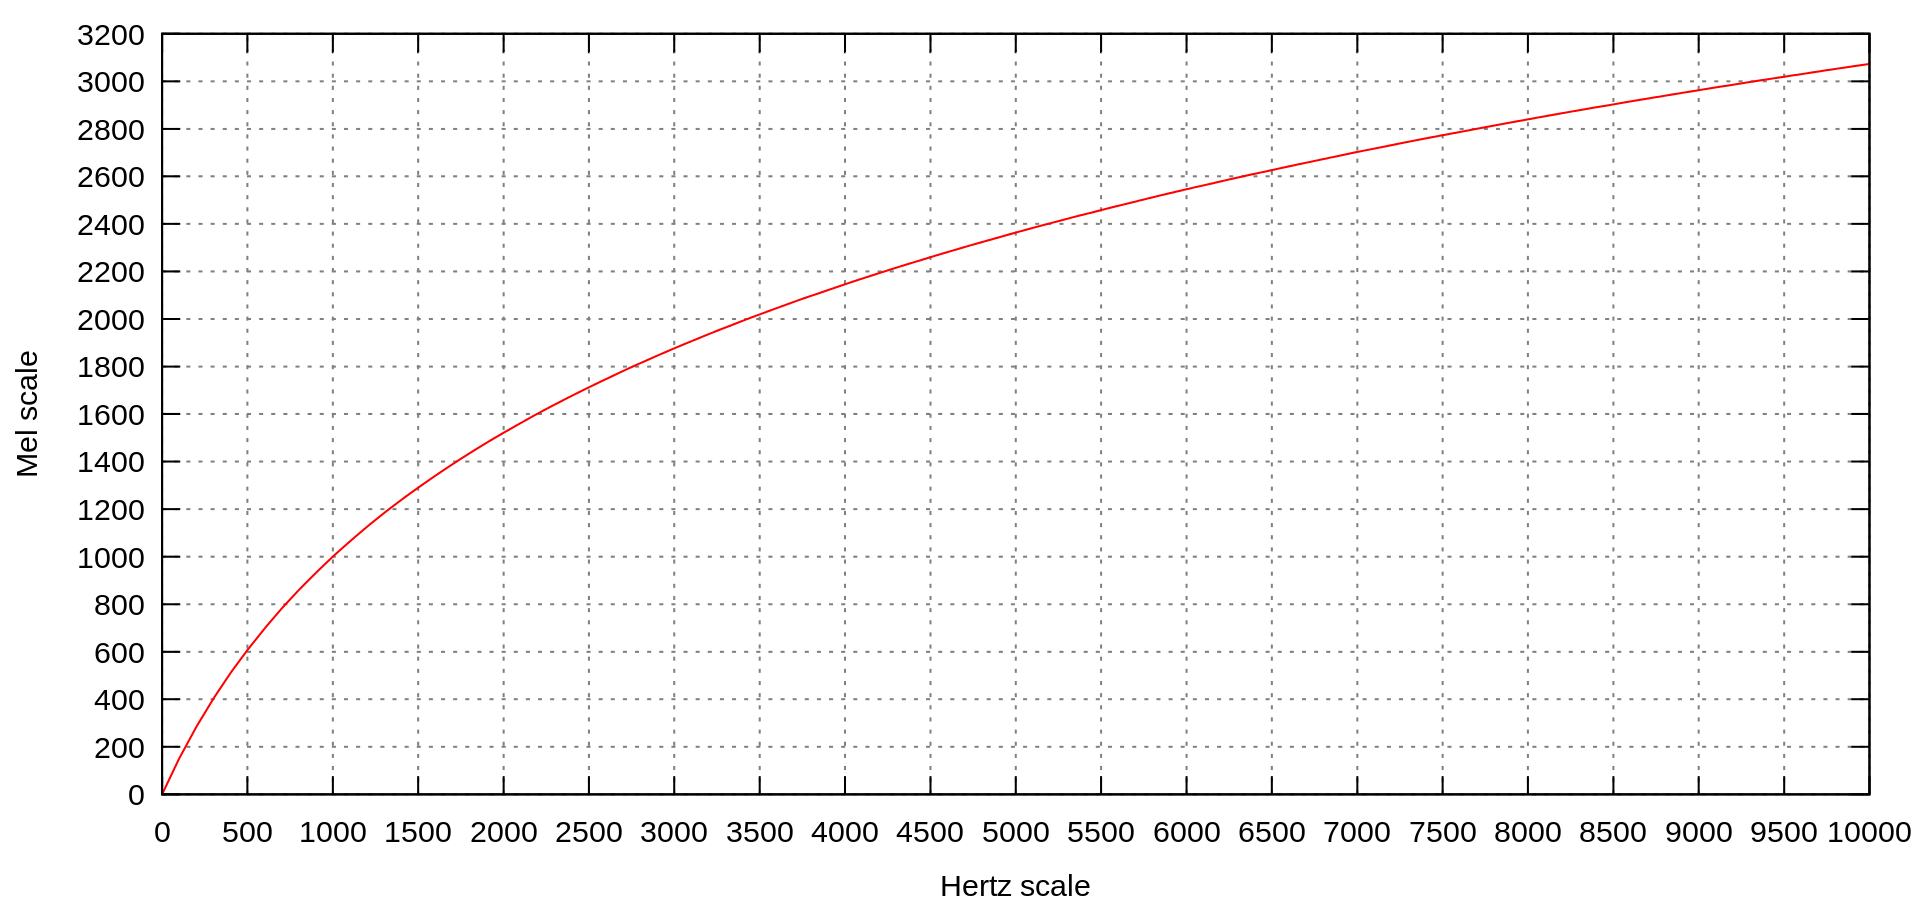
\includegraphics[width=\linewidth]{assets/Mel-Hz_plot.png}
	\caption{Мел-частотная шкала}
	\label{fig:mel-hz}
\end{figure}

Принято, что высота звука частотой 1000 Гц при уровне 40 дБ равна 1000 мел. \cite{mel} Перевод частоты из герц в мел осуществляется по формуле \ref{eq:mel}:
\begin{equation}\label{eq:mel}
    Mel(f) = 2595 \cdot \log_{10} \left( 1 + \cfrac{f}{700} \right),
\end{equation}
где $f$ -- частота (Гц), $Mel$ -- частота (мел).


Гребенка фильтров для мел-частотных кесперальных коэффициентов -- набор треугольных окон в мел-шкале. Поскольку высота тонов, начиная с частоты больше 1 кГц, возрастает гораздо медленнее, высокочастотные фильтры гребенки имеют большую полосу пропускания, чем фильтры низких частот. При такой фильтрации может быть упущена значимая информация. Однако, существует комплиментарный метод, использующий обратные мел-частотные кепстральные коэффициенты.

Также набор треугольных фильтров используется в нахождении линейночастотных кепстральных коэффициентов (\textit{linear frequency cepstral coefficients}), но фильтры расположены равномерно по линейной полосе частот. Актуальность данного метода объясняется тем, что по теории речеобразования строение речевого тракта, и в частности его длина, отображается в высокочастотной области спектра, которой мало внимания уделяется при использовании мел-частотных кесперальных коэффициентов. \cite{lfcc}

\section{Динамические характеристики}
Среди динамических характеристик, применяющихся в современных системах распознавания речи можно назвать звонкость и сонорность.


\textit{Характеристика звонкости.} Использование характеристики звонкости может привести к улучшению результатов распознания за счет лучшей дифференциации фонем. Динамическая характеристика звонкости (основного тона) -- величина, выражающая насколько периоическим является речевой сигнал в момент времени $t$. Для измерения периодичности используют автокорелляционную функцию. Автокорееляция $R^t(\tau)$ выражает схожесть между временным окном и его копией, смещенной на $\tau$.

\textit{Характеристика сонорности.} Сонорность фонемы можно определить как степень участия ее шумовых составляющих. Для получения значения динамического коррелянта предлагается \cite{sonor} использовать производную спектра в частотной области (\ref{eq:son}):
\begin{equation}\label{eq:son}
    S^{(i)}_t = \log\left( \sum^{N / 2}_{n = 0}\left|a^{(i)}_t[n]\right|\right),
\end{equation}
где $a^{(i)}_t[n]$ -- производная спектра $i$-го порядка нормализованного спектра $\hat{X}_t[n]$. 
\chapter{Система распознавания речевых эмоций}
\section{Постановка задачи}
Задача заключается в выявлении эмоциональной составляющей речи по акустическим и лингвистическим признакам и распознавание смысла эмоции индивида. Эти эмоции, являясь непроизвольной реакцией индивида на попытку исследователя тем или иным образом прояснить исследуемую ситуацию, должны были бы позволить сделать заключения в отношении сказанного испытуемым и прояснить как позицию испытуемого в ситуации
дознания.

Система распознавания эмоций на основе речи соотносит исходные данные на входе -- речевой сигнал, к определённому классу на выходе -- виду эмоции, с помощью выделения существенных признаков -- речевых особенностей, характеризующих эти данные.

В работе системы можно выделить четыре основных этапа: предварительная обработка речевого сигнала, выделение его характерных особенностей, предварительная обработка особенностей речевого сигнала перед классификацией и классификация.

\section{Предварительная обработка сигнала}
Предварительная обработка включает в себя аналоговоцифровое преобразование (АЦП) входного сигнала для получения его спектральных составляющих; цифровую фильтрацию сигнала, удаление неречевых компонентов сигнала и.~т.~д. \cite{preprocess}

Под термином \textit{цифровая фильтрация} обычно понимают локальную цифровую обработку сигнала скользящим окном. При этом полагают, что размер окна много меньше размера выборки обрабатываемого фрагмента сигнала. Для каждого положения окна, за исключением, возможно, небольшого числа крайних точек выборки, выполняются однотипные действия, которые определяют отклик, или выход фильтра. Различают линейную и нелинейную цифровую фильтрацию. \cite{methodcos}

\noindentЛинейная цифровая система описывается уравнением свертки (\ref{eq:linear-filter}):
\begin{equation}\label{eq:linear-filter}
    y[n] = \sum_{l = -\inf}^{\inf} h_l\;x[n - l],
\end{equation}
где $x[n]$ -- входная выборка, $y[n]$ -- выходная выборка, $h_l$ – импульсная
характеристика системы.

Примером нелинейной цифровой фильтрации являются семейсива порядковых фильтров. Они широко используются в задачах цифровой обработки сигналов и изображений, в частности для обнаружения объектов, выделения границ, подавления импульсных помех. Отклик порядкового p -фильтра определяется как p -я порядковая статистика $[20, 24, 25]$, т. е. элемент под номером $p$ , где $p$ -- одно из чисел $\{0, 1, \cdots, N - 1\}$, где N – размер апертуры фильтра в вариационном ряду, полученном из выборки исходных данных.

Оцифрованные образцы речи сначала нормализуются. Далее образцы сегментируется на кадры продолжительностью 30 мc с перекрытием 10 мc с использованием окна Хэмминга, которое имеет следующий вид (\ref{eq:hamming}):
\begin{equation}\label{eq:hamming}
    w_n = 0,54 - 0,46\cdot\cos\left( 2\pi \cfrac{n}{N - 1}\right),\;n = 0,\cdots,N-1,
\end{equation}
где $N$ -- длина окна, выраженная в отсчетах.
\section{Предобработка характерных особенностей}
Векторы признаков, полученные на предыдущем этапе, перед подачей их на вход выбранному классификатору нормализуются; содержащие более 2–10\% нулевых значений, отбрасываются. \cite{speechrecog} Так как на большинство классификаторов негативно влияет избыточность, то для уменьшения размерности итогового вектора признаков используются различные алгоритмы выбора признаков (прямой выбор признаков, генетический алгоритм, последовательный прямой плавающий поиск).

% Одним из алгоритмов выбора признаков является \textit{генетический алгоритм}~--~метод оптимизации, основанный на биологическом процессе естественного отбора. \cite{genetic}

\section{Классификация}
Распознавание голоса отличается от многих систем распознавания тем, что в данном случае предметом является процесс, а не статическое изображение, как в случае с распознаванием, например, изображений. Поэтому чаще всего образец голоса представляется не в виде единого вектора признаков, а в виде последовательности векторов признаков, каждый из которых описывает характеристики небольшого участка
речевого сигнала. . Последовательность векторов, полученная после этапа обработки сигнала, используется для построения шаблона диктора или для осуществления сравнения с уже построенными шаблонами.
Точность классификации в значительной мере зависит от выбранного типа классификатора.
\subsection{Скрытые Марковские модели}

Основой для скрытой марковской модели является марковская цепь. Марковская цепь задаётся начальным распределением
вероятностей $p^{0}(x)$ и вероятностями перехода $T(x', x)$

$T(x', x)$ -- это распределение следующего элемента цепи в зависимости от следующего; распределение на $(t + 1)$–м
шаге описывается согласно \ref{eq:markov-chain}:
\begin{equation}\label{eq:markov-chain}
	p^{t + 1}(x') = \int T(x'; x)p^{t}(x) dx.
\end{equation}
В дискретном случае $T(x', x)$ -- это матрица вероятностей $p(x' = i\;|\;x = j)$.

Марковская модель --  статистическая модель, имитирующая работу процесса, похожего на марковский процесс с неизвестными параметрами, и задачей ставится определение неизвестных параметров на основе наблюдаемых.

\begin{figure}[H]
	\centering
	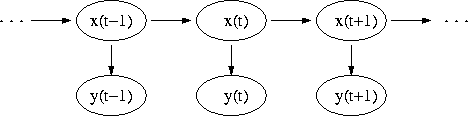
\includegraphics[width=0.85\linewidth]{assets/cmm}
	\caption{Скрытая марковская модель}
	\label{fig:cmm}
\end{figure}

На рисунке \ref{fig:cmm} $x(t)$ — сам процесс (модель), а $y(t)$ -- наблюдаемые неизвестные параметры.

Главное свойство скрытой марковской модели -- следующее состояние зависит только от предыдущего состояния \ref{eq:markov-state}:
\begin{multline}\label{eq:markov-state}
	p(x(t) = x_j \;| \; x(t - 1) = x_{j_{t - 1}}, \cdots, x(1) = x_{j_1}) = \\ 
					p(x(t) = x_{j}\;|\;x(t - 1) = x_{j_{t - 1}}). \;\;\;
\end{multline}
Здесь вероятность $a_{ij} = p(x(t) = x_j \;| \; x(t - 1) = x_{i})$ не зависит от времени $t$.
Вероятности $a_{ij}$ составляют матрицу перехода $A = (a_{ij})$.


При распознавании речи наблюдается не $x(t)$, т.~е. реальные состояния модели, а $y(t)$ -- некоторая функция от них.

%Скрытая Марковская модель состоит из последовательности состояний $S_1, S_2, S_3, \cdots$ которые связаны мгновенными вероятностными переходами $a_{ij}$, т.е. вероятность перехода из $i$~-го состояния в $i$~-ое. Возможны переходы только в следующее состояние и зацикливание. 
%
%В каждый момент времени модель осуществляет вероятностный переход из одного состояния в другое или остаётся в том же самом состоянии, при этом происходит излучение выходного акустического вектора $y_k$ с выходным вероятностным распределением $b_n(y_k)$, соответствующие этому состоянию. Эти вероятности называют \textit{эмиссионными} вероятностями. 
%
%Тогда некоторое высказывание, описываемое последовательностью акустических векторов параметров $X = \{x_1, x_2, \cdots, x_n\}$, можно промоделировать последовательностью дискретных стационарных состояний $Q = \{q_1, q_2, \cdots, q_k\},\;k\leq N$ с мгновенными переходами между этими состояниями и последовательностью излученных при этом акустических векторов $Y = {y_1, y_2, \cdots , y_N}$. \cite{markov}

\subsection{Метод k-ближайших соседей }
В качестве шаблона диктора в данном методе используется полный набор векторов обучающей последовательности. Сравнение образца с таким шаблоном происходит следующим образом: каждый вектор тестовой последовательности сравнивается с каждым вектором шаблона для определения минимального расстояния. Полученные расстояния усредняются для формирования итоговой оценки (\ref{eq:neigh}):
\begin{equation}\label{eq:neigh}
    d_k = \sum^{L}_{i = 1}\min{x_j\in S_{p_k}}d(x_i, x_j)
\end{equation}
Для снижения вычислительной трудоёмкости используют различные методы сокращения шаблона либо методы сохранения данных для ускорения поиска, такие, как, например, kd-дерево или другие методы. \cite{det}
\subsection{Модель гауссовых смесей}
Модель представляет собой взвешенную сумму Гауссиан (\ref{eq:gauss}):
\begin{equation}\label{eq:gauss}
    p(x | \lambda) = \sum^{M}_{i = 1}w_ip_i(x),
\end{equation}
где $\lambda$ -- модель диктора, $M$ -- количество компонентов модели, $w_i$ -- веса компонентов, такие, что (\ref{eq:gauss-sum}):
\begin{equation}\label{eq:gauss-sum}
     \sum^{M}_{i = 1}w_i = 1.
\end{equation}
Функция плотности вероятности каждого компонента вычисляется следующим образом:
\begin{equation}\label{eq:gauss-prob}
     p_i(x) = \cfrac{1}{(2\pi)^{\frac{D}{2}} |\Sigma_i|^{\frac{1}{2}}}
     \exp{\left(-\cfrac{1}{2}\left(x - \mu_i\right)^T\Sigma_{i}^{-1}(x - \mu_i)\right)},
\end{equation}
где $D$ -- размерность пространства признаков, $\mu_i$ -- вектор математического ожидания, $\Sigma$ — матрица ковариации.
